We present detailed analysis on our pretraining and finetuning strategy, as well as benchmark results of our two proposed detectors on three 3D detection benchmarks.




\begin{figure}[h]
    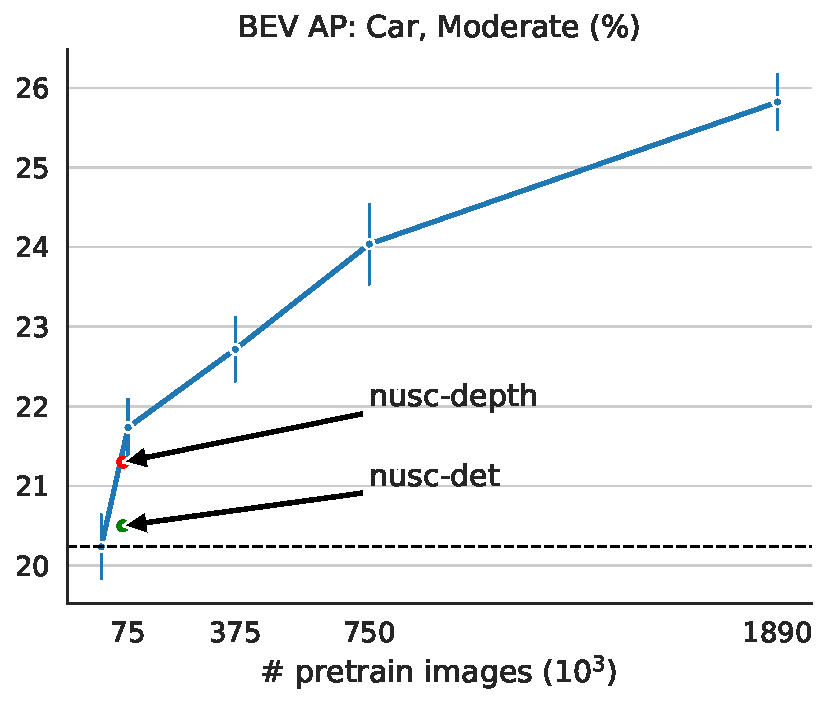
\includegraphics[width=0.99\columnwidth,trim={0mm 0mm 0mm 0mm},clip]{figures/scaling_law.pdf}
    \caption{Accuracy of 3D detection continues to improve, at least up to 1.89M images used for pre-training. We pre-train FCOS-3D with growing sizes of image-pointcloud pairs until convergence. The models are then fine-tuned on for 3D detection on KITTI \emph{train}, and evaluated on KITTI \emph{val}.}
    \label{fig:pretraining_vs_depth}
\end{figure}


\begin{table}[t!]
\centering
{
\footnotesize
\setlength{\tabcolsep}{0.4em}
\rowcolors{2}{lightgray}{white}
\begin{tabular}{l|ccc|ccc}
\toprule
& \multicolumn{3}{c}{BEV AP} & \multicolumn{3}{c}{3D AP} \\ 
\multirow{-2}{*}{Pre-train task}& 
Car & 
Pedestrian &
Cyclist &
Car & Pedestrian & Cyclist \vspace{0.5mm}\\
\midrule
%  DLA-34, Det2D & 
% 16.84 & 
% 7.01 &
% 2.88 &
% 11.20 &
% 5.64 &
% 2.40
% \\
2D-det (coco)  & 
% 16.84 & 
% 7.01 &
% 2.88 &
% 11.20 &
% 5.64 &
% 2.40
20.24 & 
7.82 &
3.77 &
13.94 &
6.01 &
3.13
\\
\midrule
% DLA-34, Depth & 
% 21.70 & 
% 9.29 &
% 3.30 &
% 15 .06 &
% 7.33 &
% 2.75
% \\
+ 2D-det (nusc) & 
x.xx & 
x.xx &
x.xx &
x.xx &
x.xx &
x.xx
\\
+ Depth  (nusc) & 
x.xx & 
x.xx &
x.xx &
x.xx &
x.xx &
x.xx
\\
\midrule
+ Depth (internal) & 
\textbf{25.82} & 
\textbf{9.93} &
\textbf{4.36} &
\textbf{18.20} &
\textbf{7.64} &
\textbf{3.75}
\\
\bottomrule
\end{tabular}\\\vspace{0mm}
\caption{We aim to ablate the role of pre-training on depth estimation via controlled experiments. We use FCOS-3D to pre-train subset of parameters relevant to each pre-train task, and fine-tine on KITTI \emph{train} for 3D detection. \textbf{2D-det} denotes 2D bounding box detection as pre-training task; \textbf{Depth} denotes supervised depth prediction using ground-truth depth available from Lidar point-cloud. Starting from parameters pre-trained on MS-COCO dataset (2D detection), we perform additional pre-training in target domain (i.e. autonomous driving) on either 2D detection or depth estimation, using the \emph{same} set of images (\textbf{nusc}) until convergence. To understand how the accuracy scales with respect to the size of pre-train data, we internally collect a large set of image-Lidar pairs (\textbf{internal}) and use it for depth pre-training. The fine-tuned models are evaluated on KITTI \emph{val}. We only report "Moderate" metrics. Depth pretraining significantly improves 3D detection accuracy, up to \textbf{30.6\%} from the baseline pre-training method.}
\label{table:dla-34}
}
\end{table}

\begin{table}[t!]
\centering
{
\footnotesize
\setlength{\tabcolsep}{0.4em}
\rowcolors{2}{lightgray}{white}
\begin{tabular}{c|ccc|ccc}
\toprule
& \multicolumn{3}{c}{BEV AP} & \multicolumn{3}{c}{3D AP} \\ 
\multirow{-2}{*}{Pre-train task}& 
Car & 
Pedestrian &
Cyclist &
Car & Pedestrian & Cyclist \vspace{0.5mm}\\
\midrule
%  DLA-34, Det2D & 
% 16.84 & 
% 7.01 &
% 2.88 &
% 11.20 &
% 5.64 &
% 2.40
% \\
2D Det. (coco)  & 
8.40 & 
2.49 &
0.09 &
4.58 &
1.70 &
0.03
\\
% \midrule
% DLA-34, Depth & 
% 21.70 & 
% 9.29 &
% 3.30 &
% 15 .06 &
% 7.33 &
% 2.75
% \\
% 2D Det. (coco + nuim) & 
%x.xx & 
%x.xx &
%x.xx &
%x.xx &
%x.xx &
%x.xx
%\\
%Depth & 
%x.xx & 
%x.xx &
%x.xx &
%x.xx &
%x.xx &
%x.xx
%\\
  + Depth & 
\textbf{24.27} & 
\textbf{9.59} &
\textbf{3.34} &
\textbf{17.34} &
\textbf{8.17} &
\textbf{2.65}
\\
\bottomrule
\end{tabular}\\\vspace{0mm}
\caption{Pre-training on supervised depth estimation allows for training larger backbone of FCOS-3D. We pre-train V2-99 \cite{lee2019centermask} backbone (96.9M parameters) using 2D detection on MS-COCO dataset, and perform additional pre-training using depth prediction on our internal dataset of image-pointcloud pairs. The models are then fine-tuned on KITTI \emph{train} for 3D detection, and evaluated on KITTI \emph{val}. The depth pre-training significantly improve rare classes: 4$\times$ for "Pedestrian", 37$\times$ for "Cyclist". We run each fine-tuning experiment four times, and report the average. We only report "Moderate" metrics due to limited space.}
\label{table:v2-99}
}
\end{table}

\subsection{3D detection}
\label{subsec:3d_detection}

\noindent\textbf{KITTI3D} Our numbers on the \textit{validation split} of the KITTI3D dataset are summarized in Table~\ref{table:kitti_3d_val} for the BEV and 3D detection tasks. We note that our baseline numbers are on par with related methods, and we record a significant increase in performance when using the modifications proposed in this paper. Our baseline FCOS-3D model uses COCO~\cite{lin2014microsoft} pretraining and we record an increase of $22\%$ by using depth estimation as an auxiliary task for pretraining ($17.03$ vs $13.96$). Our PL numbers improve over the current state-of-the-art on this split by $58\%$ and over our baseline by $75\%$ ($22.31$ vs $14.10$ and $12.68$ respectively). Note that we are omitting from this comparison the results reported by methods that use depth trained on images that overlap with the KITTI3D train and val splits. 

% , as discussed in detail in Sec.~\ref{subsec:eigen_clean}, e.g.~\cite{weng2019monocular,ma2019accurate,ding2020learning}.

Our numbers on the \textit{test split} of the KITTI3D dataset are reported in Table~\ref{table:kitti_3d_test}. Our novel single-stage 3D detector (\textit{FCOS-3D}) outperforms all other single and two-stage detectors, with a notable improvement of $21\%$ over the previous best published results for the Car - Easy category (i.e. in 3DAP $20.09$ vs. $15.54$); our improvements are significantly more noticeable on smaller classes (i.e. cyclists and pedestrians), as reported in the supplementary. Our PL-based detector also outperforms the previous state-of-the-art in this category by a significant margin - for Car - medium our 3DAP is $11\%$ higher (i.e. $13.05$ vs $11.72$). We ablate the various components of our method in Sec.~\ref{subsec:ablative_analysis}.


\begin{table}[t!]
\centering
{
\footnotesize
\setlength{\tabcolsep}{0.4em}
\rowcolors{2}{lightgray}{white}
\begin{tabular}{l|ccc|ccc}
\toprule
& \multicolumn{3}{c}{BEV AP} & \multicolumn{3}{c}{3D AP} \\ 
\multirow{-2}{*}{Depth net}& 
Easy & 
Med &
Hard &
Easy & Med & Hard \vspace{0.5mm}\\
\midrule
% ROI-10D~\cite{manhardt2019roi} & 
% 9.78 & 
% 4.91 &
% 3.74 &
% 4.32 &
% 2.02 &
% 1.46
% \\
% GS3D~\cite{li2019gs3d} & 
% 8.41 & 
% 6.08 &
% 4.94 &
% 4.47 &
% 2.90 &
% 2.47
% \\
MonoGRNet~\cite{qin2019monogrnet} & 
19.72 & 
12.81 &
10.15 &
11.90 &
7.56 &
5.76
\\

% MonoPSR~\cite{ku2019monocular} & 
% 18.33 & 
% 12.58 &
% 9.91 &
% 10.76 &
% 7.25 &
% 5.85
% \\

% SS3D~\cite{jorgensen2019monocular} & 
% 16.33 & 
% 11.52 &
% 9.93 &
% 10.78 &
% 7.68 &
% 6.51
% \\

MonoDIS (single)~\cite{simonelli2019disentangling} & 
18.45 & 
12.58 &
10.66 &
11.06 &
7.60 &
6.37
\\

M3D-RPN~\cite{brazil2019m3d} & 
20.85 & 
15.62 &
11.88 &
14.53 &
11.07 &
8.65
\\

% SMOKE~\cite{liu2020smoke} & 
% 20.83 & 
% 14.49 &
% 12.75 &
% 14.03 &
% 9.76 &
% 7.84
% \\

MonoPair~\cite{chen2020monopair} & 
24.12 & 
18.17 &
15.76 &
16.28 &
12.30 &
10.42
\\

MonoDIS (multi)~\cite{simonelli2020disentangling} & 
23.40 & 
17.20 &
15.30 &
16.50 &
12.20 &
10.30
\\

Kinematic3D~\cite{brazil2020kinematic} & 
27.83 & 
19.72 &
15.10 &
19.76 &
14.10 &
10.47
\\

\midrule

Baseline: FCOS-3D & 
%26.72 &
%19.97 &
%16.49 &
%19.23 &
%13.96 &
%11.11 
26.77 &
20.24 &
16.72 &
18.84 &
13.94 &
11.25 
\\

Ours: FCOS-3D & 
% 32.02 &
% 24.06 &
% 20.42 &
% 22.80 &
% 17.03 &
% 13.77
33.23 &
25.82 &
21.75 &
24.01 &
18.20 &
14.85
\\


% Baseline: BTS + PL & 
% 31.90 &
% 22.14 &
% 19.24 &
% 22.75 &
% 15.61 &
% 13.34 
% \\


\midrule
Baseline: PL &  % PackNet 
25.42 &	
17.97 &	
15.22 &  
18.50 & 
12.68 & 
10.78
\\


Ours: PL &  % PackNet 
\textbf{43.46} & 
\textbf{29.96} &
\textbf{25.07} &
\textbf{34.01} &
\textbf{22.31} &
\textbf{18.58} 
\\

% Ours: BTS + PL & 
% 31.90 &
% 22.14 &
% 19.24 &
% 22.75 &
% 15.61 &
% 13.34 
% \\



\bottomrule
\end{tabular}\\\vspace{0mm}
\caption{
\textbf{3D detection performance on the KITTI3D validation set} for the Car category using the AP$|_{R_{40}}$ metric.}
\label{table:kitti_3d_val}
}
\end{table}


\begin{table}[t!]
\centering
{
\footnotesize
\setlength{\tabcolsep}{0.4em}
\rowcolors{2}{lightgray}{white}
\begin{tabular}{l|ccc|ccc}
\toprule
& \multicolumn{3}{c}{BEV AP} & \multicolumn{3}{c}{3D AP} \\ 
\multirow{-2}{*}{Depth net}& 
Easy & 
Med &
Hard &
Easy & Med & Hard \vspace{0.5mm}\\
\midrule
ROI-10D~\cite{manhardt2019roi} & 
9.78 & 
4.91 &
3.74 &
4.32 &
2.02 &
1.46
\\
GS3D~\cite{li2019gs3d} & 
8.41 & 
6.08 &
4.94 &
4.47 &
2.90 &
2.47
\\
MonoGRNet~\cite{qin2019monogrnet} & 
18.19 & 
11.17 &
8.73 &
9.61 &
5.74 &
4.25
\\
MonoPSR~\cite{ku2019monocular} & 
18.33 & 
12.58 &
9.91 &
10.76 &
7.25 &
5.85
\\

SS3D~\cite{jorgensen2019monocular} & 
16.33 & 
11.52 &
9.93 &
10.78 &
7.68 &
6.51
\\

MonoDIS (single)~\cite{simonelli2019disentangling} & 
17.23 & 
13.19 &
11.12 &
10.37 &
7.94 &
6.40
\\

M3D-RPN~\cite{brazil2019m3d} & 
21.02 & 
13.67 &
10.23 &
14.76 &
9.71 &
7.42
\\

SMOKE~\cite{liu2020smoke} & 
20.83 & 
14.49 &
12.75 &
14.03 &
9.76 &
7.84
\\

MonoPair~\cite{chen2020monopair} & 
19.28 & 
14.83 &
12.89 &
13.04 &
9.99 &
8.65
\\



Kinematic3D~\cite{brazil2020kinematic} & 
26.99 & 
17.52 &
13.10 &
19.07 &
12.72 &
9.17
\\

MonoDIS (multi)~\cite{simonelli2020disentangling} & 
24.45 & 
19.25 &
16.87 &
16.54 &
12.97 &
11.04
\\




Ours FCOS-3D & 
%\textbf{29.03} & 
%\textbf{19.63} &
%\textbf{16.78} &
%\textbf{20.09} &
%\textbf{13.04} &
%\textbf{11.02}
\textbf{29.41} & 
\textbf{19.59} &
\textbf{16.95} &
\textbf{20.90} &
\textbf{13.48} &
\textbf{11.27}
\\




\midrule


MonoPL$\dagger$~\cite{weng2019monocular} & 
0.0 & 
0.0 &
0.0 &
10.76 &
7.50 &
6.10
\\


AM3D$\dagger$~\cite{ma2019accurate} & 
25.03 & 
17.32 &
14.91 &
16.50 &
10.74 &
9.52
\\


PatchNet$\dagger$ ~\cite{ma2020rethinking} & 
22.97 & 
16.86 &
14.97 &
15.68 &
11.12 &
10.17
\\


\textit{RefinedMPL$\dagger$ ~\cite{vianney2019refinedmpl}} & 
\textit{28.08} & 
\textit{17.60} &
\textit{13.95} &
\textit{18.09} &
\textit{11.14} &
\textit{8.96}
\\


D4LCN$\dagger$~\cite{ding2020learning} & 
22.51 & 
16.02 &
12.55 &
16.65 &
11.72 &
9.51
\\

\textit{Demystifying$\dagger$~\cite{simonelli2020demystifying}} & 
\textit{-} & 
\textit{-} &
\textit{-} &
\textit{23.66} &
\textit{13.25} &
\textit{11.23}
\\


Ours PL & 
\textbf{28.87} & 
\textbf{18.57} &
\textbf{15.74} &
\textbf{20.78} &
\textbf{13.05} &
\textbf{10.66}
\\


\bottomrule
\end{tabular}\\\vspace{0mm}
\caption{
\textbf{3D detection performance on the KITTI3D test set} for the Car category using the AP$|_{R_{40}}$ metric. $\dagger$ denotes pseudo-lidar based methods.}
\label{table:kitti_3d_test}
}
\end{table}

\begin{table}[t!]
\centering
{
\footnotesize
\setlength{\tabcolsep}{0.4em}
\rowcolors{2}{lightgray}{white}
\begin{tabular}{l|ccc|ccc}
\toprule
& \multicolumn{3}{c}{Pedestrian} & \multicolumn{3}{c}{Cyclist} \\ 
\multirow{-2}{*}{Methods}& 
Easy & 
Med &
Hard &
Easy & Med & Hard \vspace{0.5mm}\\
\midrule
OFTNet~\cite{} &
1.28 &
0.81 &
0.51 &
0.36 &
0.16 &
0.15 
\\
SS3D~\cite{} &
2.48 &
2.09 &
1.61 &
3.45 &
1.89 &
1.44 
\\
M3D-RPN~\cite{} &
5.65 &
4.05 &
3.29 &
1.25 &
0.81 &
0.78 
\\
MonoPSR~\cite{} &
7.24 &
4.56 &
4.11 &
\textbf{9.87} &
\textbf{5.78} &
\textbf{4.57} 
\\
MonoDIS (multi)~\cite{simonelli2020disentangling} & 
9.07 & 
5.81 &
5.09 &
1.47 &
0.85 &
0.61
\\
\midrule
FCOS-3D & 
\textbf{15.86} & 
\textbf{10.49} &
\textbf{9.06} &
5.00 &
3.06 &
2.56
\\
\bottomrule
\end{tabular}\\\vspace{0mm}
\caption{
Multiclass 3D detection on KITTI3D test set. We report BEV AP$|_{R_{40}}$ metrics for "Pedestrian" and "Cyclist" category. FCOS-3D outperforms most of other approaches, with \textbf{80.5\%} improvement from the previous best method on "Pedestrian".}
\label{table:kitti_3d_test_multi_class}
}
\end{table}

\subsection{Depth estimation}
\label{subsec:depth_estimation}


\begin{table}[t!]
\renewcommand{\arraystretch}{1.00}
\centering
{
\small
\setlength{\tabcolsep}{0.4em}
\rowcolors{2}{lightgray}{white}
\begin{tabular}{l|cccc}
\toprule
% \multirow{2}{*}{\textbf{Method}} &
% \multicolumn{3}{|c|}{Lower is better $\downarrow$} &
% \multicolumn{3}{|c}{Higher is better $\uparrow$} \\
Method & 
Abs.Rel$\downarrow$ &
Sqr.Rel$\downarrow$ &
RMSE$\downarrow$ &
$\delta_{1.25}\uparrow$ 
% a2 &
% a3
\\
\toprule

Kuznietsov et al. \cite{kuznietsov2017semi}
% & 0.113 & 0.741 & 4.621 & 0.862 & 0.960 & 0.986
& 0.113 & 0.741 & 4.621 & 0.862 
\\
Gan et al. \cite{Gan2018MonocularDE}
% & 0.098 & 0.666 & 3.933 & 0.890 & 0.964 & 0.985
& 0.098 & 0.666 & 3.933 & 0.890
\\
Guizilini et al. ~\cite{packnet-semisup}
% & 0.078 & 0.378 & 3.330 & 0.927 & --- & ---
& 0.078 & 0.378 & 3.330 & 0.927 
\\
Fu et al. \cite{fu2018deep}
% & 0.072 & 0.307 & 2.727 & 0.932 & 0.984 & 0.994
& 0.072 & 0.307 & 2.727 & 0.932
\\
Yin et al. \cite{Yin2019enforcing}
% & 0.072 & --- & 3.258 & 0.938 & 0.990 & 0.998
& 0.072 & --- & 3.258 & 0.938 
\\
Lee et al. ~\cite{lee2019big} 
% & 0.059 & 0.245 & 2.756 & 0.956 & 0.993 & 0.998
& 0.059 & 0.245 & 2.756 & 0.956
\\

\midrule

Ours PackNet 
% & 0.053 & 0.179 & 2.301 & 0.968 & 0.996 & 0.999
& 0.053 & 0.179 & 2.301 & 0.968
\\
Ours BTS
% & 0.051 & 0.166 & 2.234 & 0.972 & 0.996 & 0.999
& 0.051 & 0.166 & 2.234 & 0.972
\\

\bottomrule

\end{tabular}
}
\caption{\textbf{Depth estimation results on the KITTI dataset}, for the \textit{Eigen} test split \cite{eigen2014depth} and distances up to 80m.} 
\label{table:depth_kitti}

\end{table}



\noindent{\textbf{KITTI.}} To better quantify the performance of our depth estimation component as well as place is within context, we perform experiments on the standard monocular depth estimation benchmark using the KITTI dataset. We report results with both the PackNet and BTS network architectures: we first pre-train on the $25K$ image split, and subsequently fine-tune on the Eigen train split; we report results on the Eigen test split. The exact training protocol is described in detail in the supplementary. Our results are summarized in Table~\ref{table:depth_kitti}. We compare against the current state-of-the-art and note that while other methods use ImageNet pretraining, our depth pretraining significantly improves performance by up to $30\%$ for some metrics ($0.166$ vs $0.245$ \textit{Sqr.Rel}). Our numbers indicate the our monocular depth results outperform all other published methods to date by a large margin. 

\subsection{A critical analysis of depth estimation metrics}
\label{subsec:depth_metrics}

\subsection{The impact of data on depth and 3D detection}
\label{subsec:depth_pretraining}

\begin{figure*}[t!]
% \vspace{-1mm}
\centering

\subfloat{
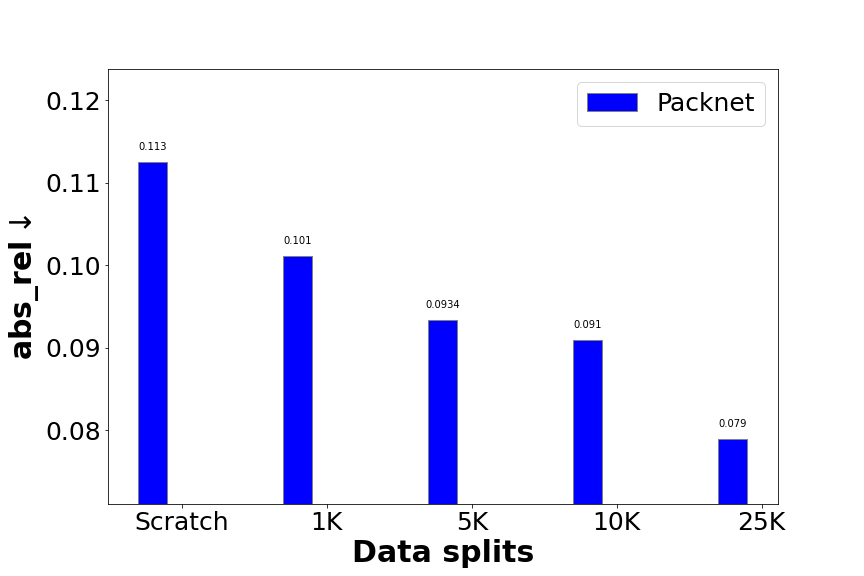
\includegraphics[width=0.3\linewidth]{figures/scaling_laws/PacknetFT_depth_metrics_k3d_val_abs_rel.png}
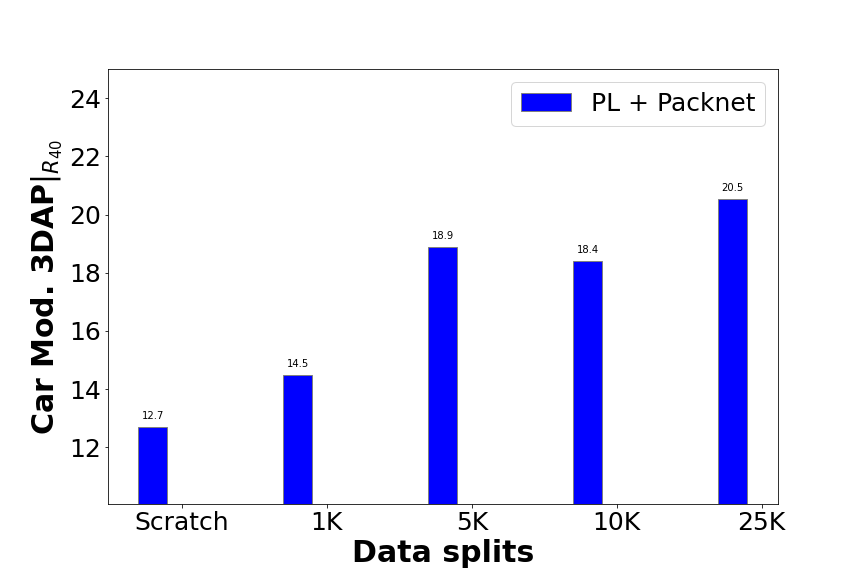
\includegraphics[width=0.3\linewidth]{figures/scaling_laws/Packnet_3d_det.png}
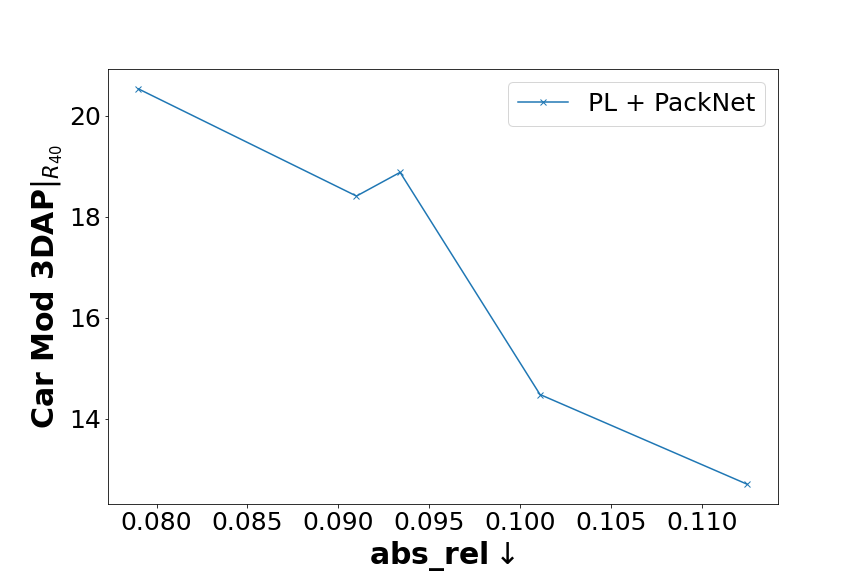
\includegraphics[width=0.3\linewidth]{figures/scaling_laws/depth_vs_3d_det_AP_3d_metrics_Mod.png}
}
\caption{
\textbf{Depth quality vs 3D AP for varying dataset sizes.} \textbf{Left:} we report the proposed \textit{abs\_rel} per-object depth metric on the KITTI3D validation split; the depth network is pretrained with varying dataset sizes and fine-tuned on the KITTI Eigen-clean split. \textbf{Middle:} for each depth network, a PL 3D detector is trained on KITTI 3D train and evaluated on KITTI 3D val. \textbf{Right:} we plot the proposed abs\_rel metric vs the resulting 3D AP metric; note that both are computed on the KITTI 3D validation split.
}
\label{fig:scaling_laws_packnet}
\end{figure*}

% -------------------------------------------------
% \begin{figure}[h]
%     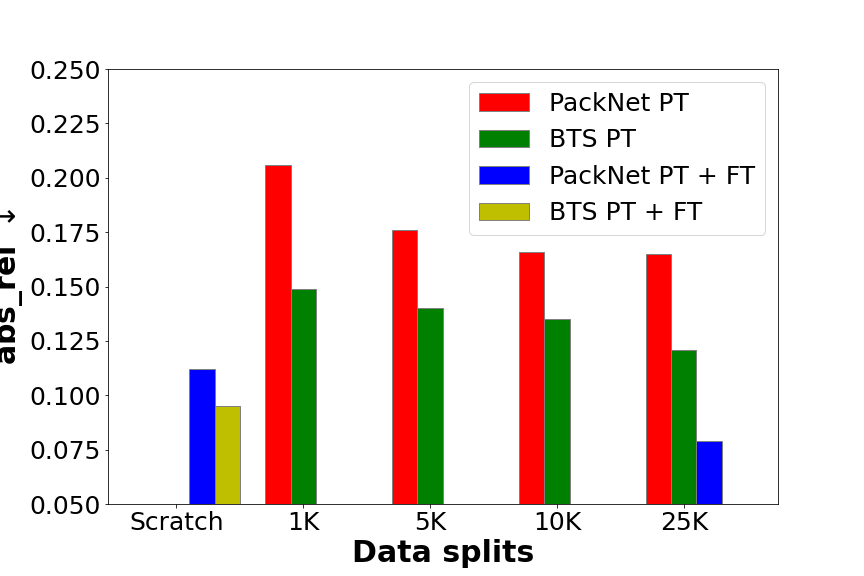
\includegraphics[width=0.99\columnwidth,trim={0mm 0mm 0mm 0mm},clip]{figures/depth_ft_transfer.png}
%     \caption{\textbf{Depth metrics on the KITTI3D validation set}: we report results for the $abs\_rel$ metric for the PackNet and BTS architectures after pre-training on varying dataset sizes. \textbf{PT} denotes pure transfer after pretraining, while \textbf{PT + FT} denotes pretraining and fine-tuning on the KITTI Eigen clean split.}
%     \label{fig:pretraining_vs_depth}
% \end{figure}

% \begin{figure}[h]
%     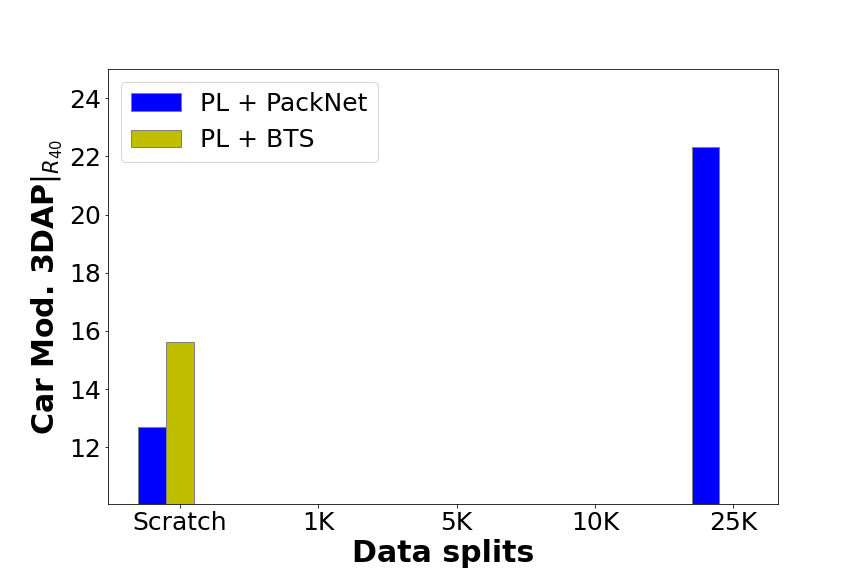
\includegraphics[width=0.99\columnwidth,trim={0mm 0mm 0mm 0mm},clip]{figures/pretraining_3d_det.png}
%     \caption{\textbf{Moderate Car 3D AP results on the KITTI validation set for the PL and FCOS3D detectors.} The depth networks are pretrained on varying dataset sizes and fine-tuned on the KITTI Eigen clean split.}
%     \label{fig:pretraining_vs_3D_det}
% \end{figure}

\subsection{Ablative analysis}
\label{subsec:ablative_analysis}


\begin{table}[t!]
\centering
{
\footnotesize
\setlength{\tabcolsep}{0.4em}
\rowcolors{2}{lightgray}{white}
\begin{tabular}{l|ccc|ccc}
\toprule
& \multicolumn{3}{c}{BEV AP} & \multicolumn{3}{c}{3D AP} \\ 
\multirow{-2}{*}{Depth net}& 
Easy & 
Med &
Hard &
Easy & Med & Hard \vspace{0.5mm}\\
\midrule
PackNet & 
41.59 & 
27.75 &
23.69 &
30.91 &
20.53 &
17.25
\\
PackNet + 2D masks  & 
40.46 & 
27.64 & 
23.03 &
32.39 &
21.29 & 
17.97 
\\

PackNet + Gauss. masks &
43.46 &
29.96 &
25.07 &
34.01 &
22.31 &
18.58 
\\



\bottomrule
\end{tabular}\\\vspace{0mm}
\caption{
\textbf{Ablative analysis of 3D detection performance with different depth fine-tuning strategies.}}
\label{table:baseline_depth_detection}
}
\end{table}





